%%%%%%%%%%%%%%%%%%%%%%%%%%%%%%%%%%%%%%%%%%%%%%%%%%%%%%%%%%
% A Template for "How to create a WiFi account" with Re2o
%
% https://gitlab.federez.net/federez/re2o/
%
% Created by Hugo 'klafyvel' Levy-Falk
% Adapted from LianTze Lim poster 
% https://www.overleaf.com/latex/examples/overleaf-campus-challenge-2016-poster/wywxgwqgtycw
% Images belong to their authors
%
% Distributed under Creative Commons CC BY 4.0
%%%%%%%%%%%%%%%%%%%%%%%%%%%%%%%%%%%%%%%%%%%%%%%%%%%%%%%%%%


% Here you can set the color and the text size
% Rézo Metz : 1cc0fa
% Aurore : cf0f23
\documentclass[color=1cc0fa, size=12pt]{re2o-poster}

\newcommand{\intranet}[1]{\newcommand{\theintranet}{#1}\newcommand{\thecontact}{#1/contact/}}
\newcommand{\email}[1]{\newcommand{\theemail}{#1}}
\newcommand{\website}[1]{\newcommand{\thewebsite}{#1}}
\newcommand{\wifi}[1]{\newcommand{\thewifi}{'#1'}}

% Set the language here
% To add another translation, create a Re2oPoster-<Lang>.dict
\usepackage[french]{babel}
\usepackage[french]{translator}
\usedictionary{Re2oPoster}

% Some informations
\title{\translate{Poster Title}}
\intranet{https://re2o.rezometz.org}
\website{https://rezometz.org}
\email{contact@rezometz.org}
\wifi{Bienvenue}

% You should not need to change anything below

\usepackage[utf8]{inputenc}
\usepackage[T1]{fontenc}

\usepackage{tabularx}
\usepackage{multicol}
\usepackage{qrcode}
\usepackage{cclicenses}

\graphicspath{{images/}}

\begin{document}

\maketitle

\vskip \baselineskip
\begin{minipage}[0.6\pageheight]{\linewidth}
\begin{multicols}{2}
\Large 
\begin{enumerate}
    \item \translate{connect};
    \item \translate{go to intranet} :
\begin{center}
\qrcode[height=0.3\linewidth]{\theintranet}
\end{center}
    \item \translate{if don't have an account}
    \item \translate{if have an account};
    \item \translate{go to your user page}; 
        \begin{itemize}
            \item {\centering%
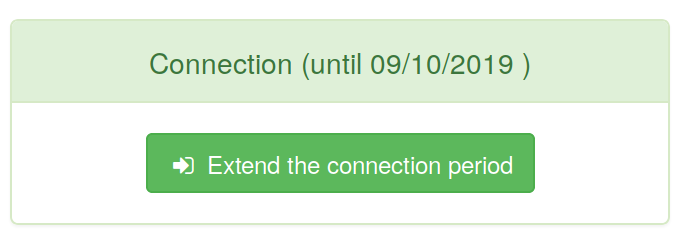
\includegraphics[width=.55\linewidth]{pane_ok.png}}

            \translate{is active}
            
            
            \item {\centering%
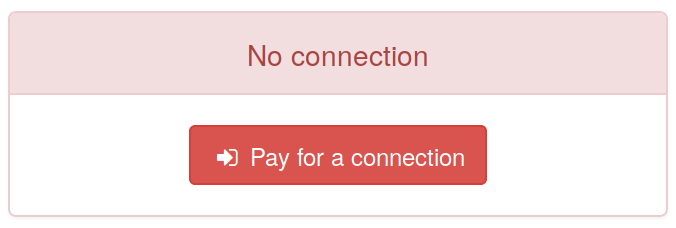
\includegraphics[width=.55\linewidth]{pane_nok.png}}

            \translate{is not active}
        \end{itemize}
    \item \translate{pay}
    \begin{enumerate}
        \item \translate{select pay} : 
        
        {\centering%
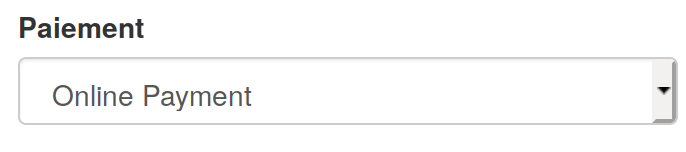
\includegraphics[width=.55\linewidth]{pay_method.png}}

        \item \translate{select article}
        
        {\centering%
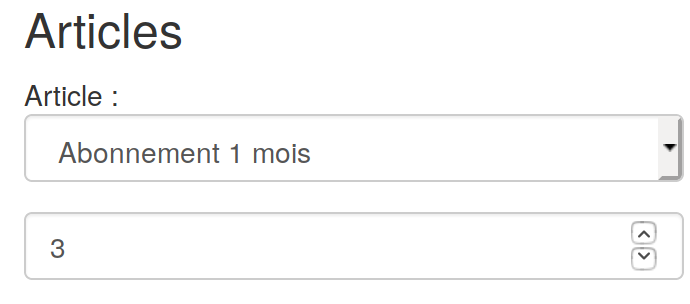
\includegraphics[width=.55\linewidth]{pay_article.png}}

        \item \translate{click}
    \end{enumerate}
    \item \translate{you can}
    
\end{enumerate}

\end{multicols}
\end{minipage}

\vskip \baselineskip

\hskip -1.1cm%
\renewcommand{\arraystretch}{1.8}%
\begin{tabularx}{\paperwidth}{%
   @{} p{1.5cm} @{}
   *4{>{\centering\arraybackslash\large\bfseries}X @{}}
   p{1.5cm} @{}
}
\rowcolor{gray!30}
\rule{0pt}{2.2cm} & 

\includegraphics[height=1.8cm]{utorrent.png} &

\includegraphics[height=1.8cm]{law.png} &

\includegraphics[height=1.8cm]{share.png} &

\includegraphics[height=1.8cm]{fun.png} & \\
& \translate{p2p} & \translate{law} & \translate{share} & \translate{enjoy}
\end{tabularx}

\hfill
{\Large \translate{issue} \emph{\thecontact}\\\hfill \translate{mail} \emph{\theemail}}

\vfill
\vskip -0.9\baselineskip
{
\footnotesize
u-torrent logo \cc\ccby FlatArt, %
law icon by Github (MIT license), %
user-icon \cc\ccby\ccsa Daniel Bruce, %
Party icon by Webalys
}

\end{document}